\documentclass[11pt]{article}
\usepackage{geometry,marginnote} % Pour passer au format A4
\geometry{hmargin=1cm, vmargin=1.5cm} % 

% Page et encodage
\usepackage[T1]{fontenc} % Use 8-bit encoding that has 256 glyphs
\usepackage[english,french]{babel} % Français et anglais
\usepackage[utf8]{inputenc} 

\usepackage{lmodern}
\usepackage[np]{numprint}
\setlength\parindent{0pt}

% Graphiques
\usepackage{graphicx,float,grffile}
\usepackage{tikz,pst-eucl,pst-plot,pstricks,pst-node,pstricks-add,pst-fun,pgfplots} 

% Maths et divers
\usepackage{amsmath,amsfonts,amssymb,amsthm,verbatim,scratch3}
\usepackage{multicol,enumitem,url,eurosym,gensymb,tabularx}

\DeclareUnicodeCharacter{20AC}{\euro}



% Sections
\usepackage{sectsty} % Allows customizing section commands
\allsectionsfont{\centering \normalfont\scshape}

% Tête et pied de page
\usepackage{fancyhdr} \pagestyle{fancy} \fancyhead{} \fancyfoot{}

%\fancyfoot[L]{Collège Faubert}
%\fancyfoot[C]{\thepage / 6}
%\fancyfoot[R]{Série Générale}

\renewcommand{\headrulewidth}{0pt} % Remove header underlines
%\renewcommand{\footrulewidth}{0pt} % Remove footer underlines

\newcommand{\horrule}[1]{\rule{\linewidth}{#1}} % Create horizontal rule command with 1 argument of height

\newcommand{\Pointilles}[1][3]{%
  \multido{}{#1}{\makebox[\linewidth]{\dotfill}\\[\parskip]
}}

\newtheorem{Definition}{Définition}

\usepackage{siunitx}
\sisetup{
    detect-all,
    output-decimal-marker={,},
    group-minimum-digits = 3,
    group-separator={~},
    number-unit-separator={~},
    inter-unit-product={~}
}

\setlength{\columnseprule}{1pt}



\begin{document}


\begin{titlepage}

    \center % Center everything on the page
    
    \textsc{\LARGE Collège Faubert}\\[1cm] % Name of your university/college
    %\textsc{\Large }\\[0.5cm] % Major heading such as course name
    \textsc{\large Villefranche-sur-Saône}\\[0.5cm] % Minor heading such as course title
    
    \horrule{2px}
    
    \vspace{0.5cm}
    
    {\Huge \bfseries Brevet Blanc}\\[1cm] % Title of your document
    {\Huge \bfseries Mathématiques}\\[1cm] % Title of your document
    {\Huge  \bfseries Série Professionnelle}\\[1cm]
    {\large \bfseries Février - 2025}\\[1cm] 
    {\bfseries Durée de l'épreuve : 2h : 100 points}\\[1cm] 
    
    \horrule{2px}
    
    \vspace{0.5cm}
    
    \begin{itemize}[label={$\bullet$}]
      \item \textsc{Exercice 1} - 12 points     
      \item \textsc{Exercice 2} - 20 points 
      \item \textsc{Exercice 3} - 20 points
      \item \textsc{Exercice 4} - 19 points 
      \item \textsc{Exercice 5} - 29 points  
    \end{itemize}
    
    \vspace{0.5cm}
    
    \horrule{2px}
    
    \vspace{0.5cm}
    
    \begin{itemize}
      \item Les exercices sont indépendants. Toutes les réponses doivent être justifiées (sauf QCM).
      \item L'usage de la calculatrice de type collège est autorisé.
      \item L'usage de tout autre document est interdit. 
      \item Toute trace écrite, même incomplète sera prise en compte dans l'évaluation.
      \item L’annexe page 6 est à rendre avec la copie.
      \item Le sujet comporte 6 pages.
    \end{itemize}
    
    \vfill 
    
    \end{titlepage}

\newpage
\setcounter{page}{2}
\subsection*{Exercice 1 - 12 points }
\textbf{Il faut répondre sur la copie et non sur l'énoncé. }
\begin{figure}[H]
  \centering
  \includegraphics[width=0.85\linewidth]{qcm1-full-pro.pdf}
\end{figure}


\newpage
\subsection*{Exercice 2 - 20 points }

\begin{multicols}{2}
Le schéma ci-contre n'est pas à l'échelle. 

\begin{itemize}[label={$\bullet$}]
  \item Les points A, E et D sont alignés.
  \item Les points A, B et C sont alignés.
  \item Les droites (EB) et (DC) sont parallèles. 
\end{itemize} 

On donne :

\begin{itemize}[label={$\bullet$}]
  \item AC = 20 cm
  \item EB = 8,7 cm 
  \item BC = 4 cm
\end{itemize} \columnbreak

\begin{figure}[H]
  \centering
  \includegraphics[width=0.8\linewidth]{pro-ex2.pdf}
\end{figure}

\end{multicols}

\begin{enumerate}
  \item[1.] Calculer en centimètre (cm), la longueur AB. \\
  \item[2.] Calculer en centimètre (cm), la longueur AE. Arrondir au dixième. \\
  Indiquer le théorème utilisé. \\
  \item[3.] L'égalité $\dfrac{EB}{DC} = \dfrac{AB}{AC}$ permet de calculer la longueur DC.\\
  Indiquer le nom du théorème qui permet d'obtenir cette égalité. \\
  \item[4.] Calculer la longueur DC en centimètre (cm). Arrondir au centième.  
\end{enumerate}


\subsection*{Exercice 3 - 20 points }

Élise s'entraîne pour passer les qualifications et représenter la France en athlétisme pour une épreuve internationale de 100 m. \\

Le tableau ci-dessous regroupe la série de ses temps en secondes lors des onze dernières compétitions. \\

\begin{center}\begin{tabular}{|*{11}{c|}}
  \hline
  10,58 & 10,59 & 11,01 & 11,03 & 11,05 & 11,08 & 11,10 & 11,11 & 11,13 & 11,18 & 11,20 \\
  \hline
\end{tabular}\end{center}

\begin{enumerate}
  \item[1.] Indiquer, en secondes, le temps minimum et le temps maximum mis par Élise pour parcourir 100m. \\
  \item[2.] Déterminer, en secondes, l'étendue de cette série. \\
  \item[3.] Les résultats sont considérés comme réguliers si l'étendue est inférieur à 0,7 secondes.\\
  Indiquer si les résultats d'Élise sont réguliers. \\
  \item[4.] Déterminer, en secondes, la médiane de cette série. \\
  \item[5.] Vérifier que la moyenne de cette série, arrondie au centième de seconde, est égale à 11,01 secondes. \\
  \item[6] Pour être sélectionnée en équipe de France, les critères suivants doivent être vérifiés : 
  \begin{itemize}
    \item 50\% des temps au 100 m sont inférieurs à 11,09 secondes.
    \item La moyenne des temps au 100 m doit être inférieure à 11,05 secondes.
  \end{itemize}
  En déduire si Élise pourra être sélectionnée en équipe de France. Justifier la réponse. 
\end{enumerate}
 
\newpage
\subsection*{Exercice 4 - 19 points }

Une commune décide d’installer des grandes jardinières en bois en forme de pavés droits sur sa place principale. \\

Elle a choisi les articles suivants :

\begin{itemize}[label={$\bullet$}]
  \item 5 jardinières en bois.
  \item 5 sacs de protection géotextile.
  \item 10 sacs de terreau.
\end{itemize}

\begin{center}\textbf{Extrait du catalogue.}\end{center}

\begin{multicols}{2}
\textsc{Jardinière en bois :} \\

Traitée autoclave classe 4. \\

\textbf{Dimensions extérieures :}

$$160\,cm \times 40\,cm \times 40\,cm$$

\textbf{Dimensions intérieures :}

$$157\,cm \times 33\,cm \times 30\,cm$$

\textbf{Capacité :} 155 Litres \\

\textbf{Matériau :} Pin massif \\ 

\textbf{Poids :} 22 kg \\

Vendu sans sac géotextile \\

\textbf{Prix unitaire :} 145,00 \euro  \\

\textbf{Frais de port : } \\
\begin{itemize}[label={$\bullet$}]
  \item 1 jardinière : 12,20 \euro 
  \item 2 jardinières : 21,50 \euro 
  \item 3 jardinières : 26,30 \euro 
  \item 4 jardinières : 32,20 \euro 
  \item 5 jardinières : 39,90 \euro 
  \item 6 jardinières et plus : 46,60 \euro 
\end{itemize} \columnbreak


\textsc{Sac de protection géotextile pour jardinière} 

$$160\,cm \times 40\,cm \times 40\,cm$$

Ce sac de protection géotextile sera fixé dans votre jardinière et protégera ainsi les parois de la terre humide. \\

\textbf{Prix unitaire :} 12,90 \euro . \\

\textbf{Pas de frais de port} si votre commande inclut l'achat de jardinières. \\ \medskip


\textsc{Terreau de plantation professionnel} \\

Terreau de plantation soigneusement élaboré avec les meilleurs composants. \\

\textbf{Volume :} 70 Litres \\

\textbf{Poids :} 25 kg \\

\textbf{Prix unitaire :} 23,50 \euro  \\

\textbf{Pas de frais de port} si votre commande inclut l'achat de jardinière.
\end{multicols}

\begin{enumerate}
  \item[1.] Compléter le bon de commande en \textbf{ANNEXE 2 page 6}. \\
  \item[2.] Vérifier si, d’après les dimensions intérieures notées sur le catalogue, la jardinière possède une capacité d’environ 155 L comme indiqué. \\
  \item[3.] La commune achète 10 sacs de terreau, elle souhaite remplir complètement les 5 jardinières. Cette quantité est-elle suffisante ?
\end{enumerate}

On rappelle que $1\,L = 1\,000\,cm^3$. 

On rappelle le calcul de volume de quelques solides usuels :


\begin{figure}[H]
  \centering
  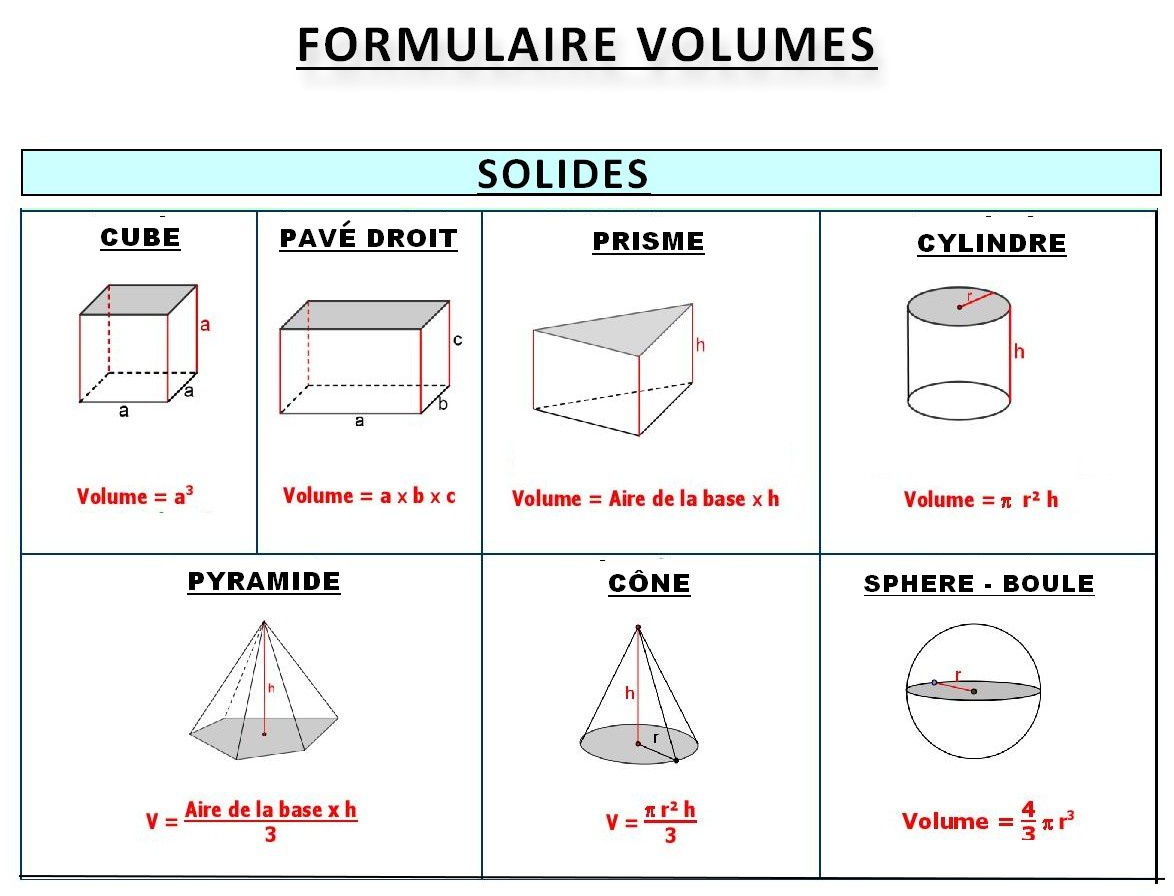
\includegraphics[width=0.8\linewidth]{pro-ex5-formu.png}
\end{figure}

\subsection*{Exercice 5 - 29 points }

Afin de se déplacer aux qualifications, le club d'athlétisme étudie les tarifs de location d'un minibus. \\

On souhaite déterminer le tarif le plus intéressant selon le nombre de kilomètres parcourus. 

\begin{itemize}
  \item \textbf{Tarif A :} 3,50~\euro{} par kilomètre.
  \item \textbf{Tarif B :} 2,50~\euro{} par kilomètre auxquels on ajoute un coût fixe de 200~\euro.
\end{itemize}

\medskip

\begin{enumerate}
  \item[1.] Calculer, en euros, le montant de la location avec le tarif A pour un trajet de 80 km. 
  \item[2.] On donne trois expressions de fonctions : 

  \[f(x) = 2,50 x \quad ; \quad g(x) = 3,50 x \quad;\quad h(x) = 3,50 x + 200\]

  Recopier sur la copie l'expression de la fonction modélisant le calcul du montant du tarif A.

  \item[3.] Placer le point N de coordonnées (160~;~560) sur le graphique en ANNEXE 1 à rendre avec la copie. 

  \item[4.] Tracer la droite passant par les points M et N. 

  On admet que la droite (MN) représente la fonction de la question 2. 

  Justifier que cette fonction est une fonction linéaire. 

  \item [5.] La droite déjà représentée en \textbf{ANNEXE 1 page 6} permet de déterminer les montants du tarif B. 

  Déterminer le nombre de kilomètres pour lequel les deux tarifs sont égaux. 

  Laisser les traits de lecture apparents sur l'\textbf{ANNEXE 1 page 6}. 

  \item[6.] Les qualifications se déroulent à une distance de 75 km du club. 

  Calculer le nombre de kilomètres effectués pour aller et revenir des qualifications. 

  \item[7.] Indiquer le tarif le plus intéressant pour le club. Justifier la réponse.
\end{enumerate}


\newpage
\textbf{Nom, Prénom : } \dotfill
\medskip \medskip

\begin{center}\textbf{ANNEXE À RENDRE AVEC LA COPIE} \end{center}




\textbf{ANNEXE 1} \\
\begin{figure}[H]
  \centering
  \includegraphics[width=0.5\linewidth]{pro-ex4.pdf}
\end{figure}

\textbf{ANNEXE 2} \\
\begin{figure}[H]
  \centering
  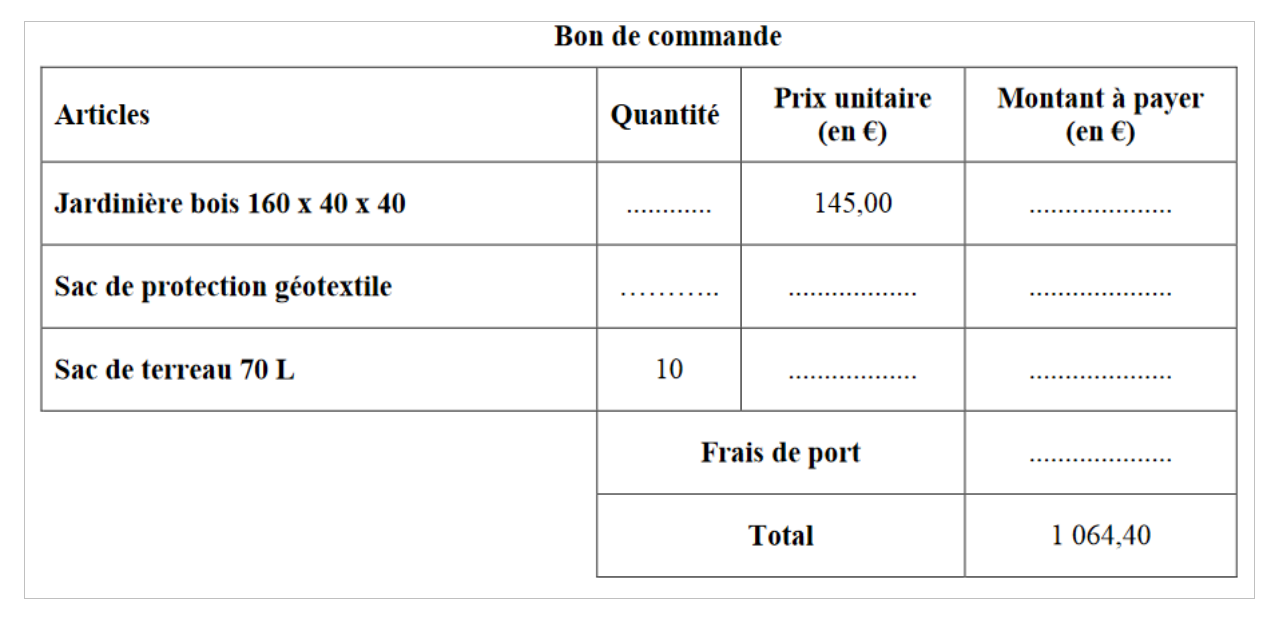
\includegraphics[width=0.7\linewidth]{pro-ex5.png}
\end{figure}

\end{document}
